\documentclass[12pt]{article}
\usepackage[utf8]{inputenc}
\usepackage[T1]{fontenc}
\usepackage[dvips]{epsfig}
%\usepackage{graphicx}
\usepackage{lineno}
\usepackage{url}

\setlength{\textwidth}{15.7cm}
\setlength{\textheight}{22cm}

\begin{document}

\title{Federated Scripting Technology in the GENESIS 3.0 Neural
  Simulation Platform}

\author{Cornelis H.$^1$ Rodriguez A. L.$^1$ Joe J. L.$^2$ Coop A. D.$^1$ Bower J. M.$^1$\\
  {\small 1. University of Texas Health Science Center at San Antonio.} \\
  {\small 2. College of Medicine, Wonkwang University, Republic of Korea.}
}

\maketitle
\pagenumbering{arabic}
\section*{Abstract}
Python is a scripting language providing a rich set of freely
available open source
libraries\,\cite{langtangen04:_python_scrip_comput_scien}. With a
clean dynamic object-oriented design producing highly readable code,
Python is widely employed in specialized areas of systems integration
(e.g\,.~\cite{thiruvathukal01:_web_progr_python}).

An important feature of the latest version of the GENESIS (GEneral
NEural SImulation System) platform, GENESIS 3 (G3), is that it
decomposes into self-contained software modules, referred to as the
CBI architecture\,\cite{cornelis08:_cbi_archit_comput_simul_realis}.
This federated architecture allows separate Python bindings to be
defined for the mathematical solvers and the GUI, as well as for other
necessary software.

Currently, there are many technologies that simplify the binding of G3
to Python libraries.  We employ SWIG (Simplified Wrapper and Interface
Generator\,\cite{08:_simpl_wrapp_inter_gener}).  SWIG examines an
application API and makes it available to a scripting language.
However, neither the API of a low-level application, nor the API
generated by SWIG possess the high-level functionality required to
complete the binding and additional code is
required\,\cite{08:_swig_python}. We employ self-query and dynamic
compilation techniques to minimize maintenance costs of existing code
and simplify addition of new functionality.

We illustrate our approach with two examples: (1) a Python script that
generates, runs, and displays the output of a simple single
compartment model neuron, and (2) the application of Python bindings
to connect the G3 simulator to Blender, an open source 3D content
creation suite.  We use these bindings to visualize 3D models based on
electron microscopy and convert them to computational
models\,\cite{cornelis08:_model_neuros_genes}.

% Abstract 1597 characters with citations replaced by [??]

\section{Introduction}

Historically, there have been fundamental differences between
scripting languages such as
Perl\,\cite{wall99:_perl_progr_refer_guide},
Python\,\cite{martelli06:_python_nutsh},
Rexx\,\cite{o'hara88:_moder_progr_using_rexx},
Tcl\,\cite{ousterhout94:_tcl_tk_toolk}, Visual Basic, and the Unix
shells and system programming languages such as C or C++.  System
programming languages start from the most primitive computer elements
such as words of memory. They are designed to manage the complexity of
building data structures and algorithms from scratch and usually
require pre-declared data types.  Alternatively, scripting languages
as a replacement for shell scripts were designed for `gluing': they
assumed the existence of a set of powerful components and were
intended primarily for connecting components together. The fact that
scripting languages are typically loosely typed and do not need a
visible compilation step simplifies connectivity between components
and allows for rapid prototyping of enterprise software systems.
%They
%are also often small, lightweight languages, suitable for embedding,
%and provide higher levels of programming in an interpreted development
%environment.
Scripting languages operate at a higher level than system programming
languages in the sense that on average a single statement does more
work. For example, a typical statement in a system programming
language executes about five machine instructions, whereas in a
scripting language hundreds or thousands of machine instructions may
be executed\,\cite{ousterhout98:_scrip}.

%9.  L. Wall, T. Christiansen, and R. Schwartz, Programming Perl, Second Edition, O'Reilly and Associates, ISBN 1-56592-149-6, 1996.
%4. M. Lutz, Programming Python, O'Reilly, ISBN 1-56592-197-6, 1996.
%6. R. O'Hara and D. Gomberg, Modern Programming Using REXX, Prentice Hall, ISBN 0-13-597329-5, 1988.
%8.  J. Ousterhout, Tcl and the Tk Toolkit, Addison-Wesley, ISBN 0-201-63337-X, 1994.
% 1. John K. Ousterhout (1998) Scripting: Higher Level Programming for the 21st Century. IEEE COMPUTER 31: 23-30.

A scripting language is not a replacement for a system programming
language or vice versa. Each is suited to a different set of tasks.
For gluing and system integration, applications can be developed
5--10x faster with a scripting language. System programming languages
require large amounts of boilerplate and conversion code to connect
the pieces, whereas this is implicit in scripting languages. Where
execution speed is key, a system programming language can often run
several orders of magnitude faster than a scripting language due to
fewer run-time checks.

The strongly typed nature of system programming languages discourages
reuse. Scripting languages, on the other hand, have actually
stimulated significant software reuse. They use a model where
interesting components are built in a system programming language and
then glued together into applications using the scripting language.
This division of labor provides a natural framework for reusability.
Components are designed to be reusable, and there are well-defined
interfaces between components and scripts that make them easy to use.
In this sense scripting and system programming are symbiotic. Used
together, they produce programming environments of exceptional power:
system programming languages are used to create functional components
which are then be assembled using scripting languages.

In summary, system programming languages are well suited to building
components where the complexity is in the data structures and
algorithms, while scripting languages are well suited for integrating
applications where the complexity is in the connections. With an
increasing requirement for software integration, scripting is
providing an important programming paradigm.

Here, we illustrate the use of the general purpose scripting languages
for making high performance simulation software coded in system
programming languages accessible to neuroscientists and biologists.

%http://en.wikipedia.org/wiki/Scripting\_languages
%Historical overview

%http://www.google.com/trends?q=perl\%2C+Python

%http://www.tiobe.com/index.php/content/paperinfo/tpci/index.html

\section{Methods \& Software}

\subsection{GENESIS}

GENESIS (GEneral NEural SImulation System) is a general purpose
simulation platform that was developed to support the simulation of
neural systems ranging from subcellular components and biochemical
reactions to complex models of single neurons, simulations of large
networks, and systems-level models. It was the first broad scale
modeling system in computational biology to encourage modelers to
develop and share model features and components. For these people, it
was the object-oriented approach taken by simulators along with their
high-level simulation languages that allowed the exchange,
modification, and reuse of models or model components. It was this
community of developers and users that ultimately drove the
development of the GENESIS platform.

GENESIS simulations are constructed from modules that receive inputs,
perform calculations on them, and then generate outputs. Model neurons
are constructed from basic components, such as compartments, and
variable conductance ion channels. Compartments are linked to their
channels and are then linked together to form multi-compartmental
neurons of any desired level of complexity. Neurons may be linked
together to form neural circuits.  It is the paradigm used by the
GENESIS SLI, the commands which it recognizes, and of the main GENESIS
`objects' which are available for constructing simulations that have
most powerfully assisted in the sharing of model features amongst the
broader modeling community.

A high-level simulation language, the GENESIS SLI, provides a
framework within which a simulation programmer can define and
manipulate GENESIS elements. It allows modelers to easily extend the
capabilities of the simulator, and to exchange, modify, and reuse
models or model components. The SLI interprets statements in the
GENESIS simulation language, and constitutes the operating system
`shell'. User-defined SLI scripts are used to glue the pieces of a
simulation together. The graphical objects used to define the front
end of a simulation and GENESIS data handlers are all controlled from
SLI scripts.

G3 is a major revision and update of the GENESIS system.  The core
simulator functionality is restructured, with a more modern modular
design (the CBI federated architecture, described below). This not
only results in improved simulator performance and portability, but
also allows the use of alternate script parsers and user interfaces,
as well as the ability to communicate with other modeling programs and
environments. The CBI federated architecture is specifically designed
to support the integration of these stand-alone software components
and applications using modern integration technologies.

The core components of the architecture are shown in
Figure~\ref{fig:cbi-arch}. On the bottom left are databases of
neuronal models or experimental data that can be accessed by the
simulator. Optional model processors (e.g. the reConstruct interface,
see below) load a model into the model container.  The model container
stores the model in memory and makes it available to other software
components in different formats.  One function of the model container
is to translate biological concepts and properties into mathematical
formulae that can be understood by the mathematical solvers. Thus,
importantly and unlike other existing neural simulators, the
mathematical solvers are independent of the biological representation
of a model. The simulation controller orchestrates and synchronizes
the actions taken by the model container (e.g. when to load a model,
the definition of the stimulus, and when to export a model) and
mathematical solvers (when to fetch the model from the model
container, when to start the calculations, and what the output
variables are).

\begin{figure}[ht]
  \centering
    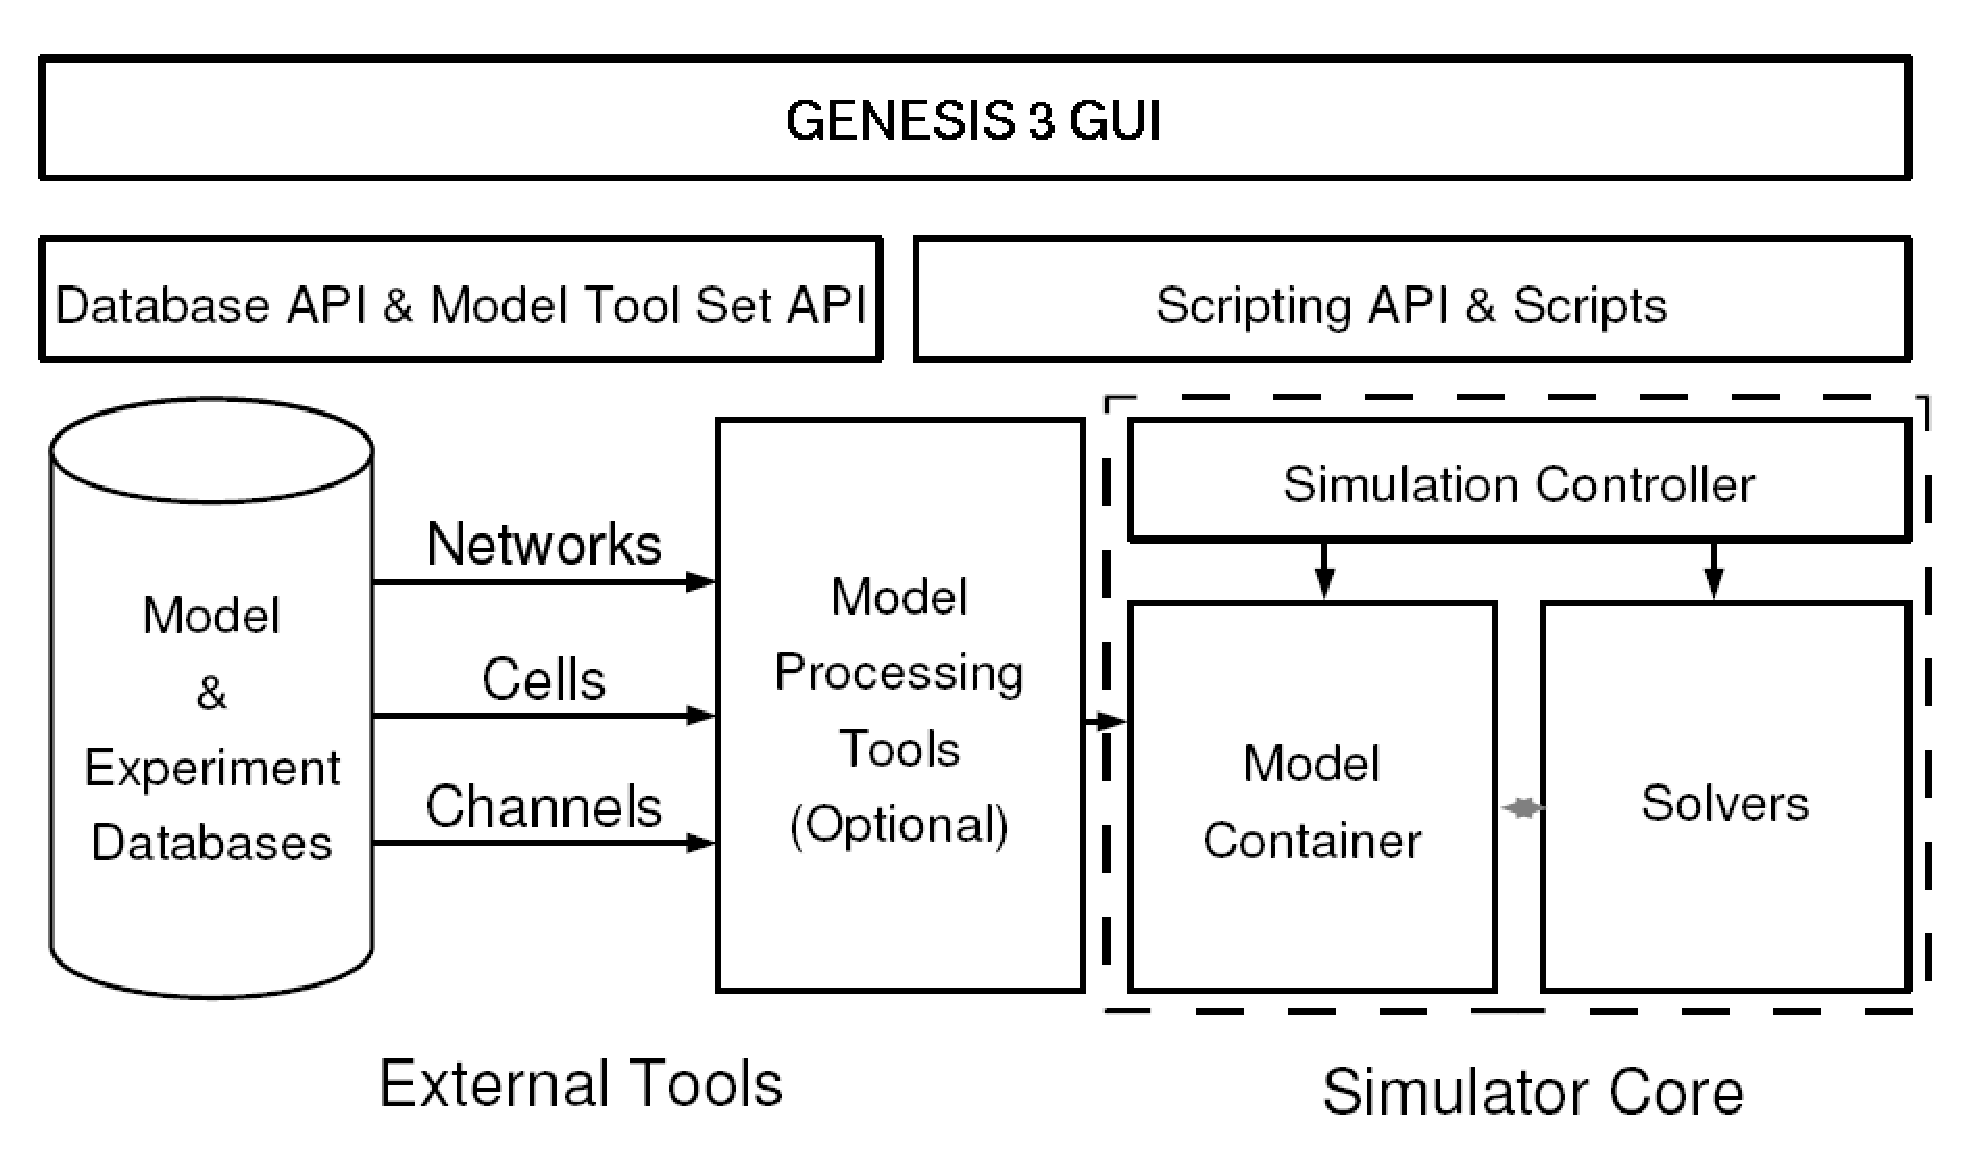
\includegraphics[scale=0.4]{figures/G3arch.eps}
  \caption{Relation of components in the CBI architecture.}
  \label{fig:cbi-arch}
\end{figure}

The scripting layer allows the simulation system to be driven from
multiple scripting languages. Python and Perl are currently supported,
and for backwards compatibility, the GENESIS SLI is being
incorporated. The G3 Graphic User Interface (GUI), shown at the top,
is entirely developed in Python.  It allows models to be imported from
databases or constructed from scratch, the exploration of model
structure and parameters, and the visualization of variables and model
behavior (see below).


\subsection{The CBI Federated Architecture}
The CBI (Computational Biology Initiative) federated architecture
provides a modular paradigm that places stand-alone software
components into logical relationships. In this it shares a number of
ideas with the well-known three-tier architecture paradigm.  The
distinguishing feature of the CBI architecture is that the back end
comprises mathematical solvers rather than relational databases.  The
data layers in the CBI architecture correspond to high-level data
associated with biological concepts and extend to low level data such
as numerical values. The benefit of this layering of data is that it
allows the mathematical and biological aspects of a model to be
distinguished and separated.

Clear delineation of the modules in the CBI architecture allows both
developers and users to choose to contribute to a single component
with limited complexity, instead of being forced to contribute to the
whole simulator and be exposed to tremendous complexity. Within the
CBI paradigm each software component is self contained in the sense
that it can be run independently. This facilitates the
interoperability of software obtained from different sources and has
several important advantages, including: (1) reduced complexity of
software modules compared to a unitary system, (2) simplified
documentation of modules in terms of inputs and outputs, (3) easy
incorporation or removal of individual modules as required, (4)
simplified development and testing of components as stand alone
modules, and (5) clear delineation of scope for the development of new
modules. The federated approach provides three significant advantages
for software development: (1) modules can be run separately on
different machines, for example, the GUI and modeling environment
might run locally, while the simulator runs elsewhere, either serially
or in parallel, on more powerful machines, (2) decomposition of an
application into multiple software components allows reuse and
extension of individual modules, whether stand alone or otherwise,
clearly facilitating model development and research progress, and (3)
individual components can be independently updated, enhanced, or
replaced when needed, thus the life cycle of a modular architecture is
smoother than that of a non-scalable application.

The Neurospaces project provides core software components of the G3
neuroscience simulator\,\cite{cornelis03:_neuros} including, (1) the
{\it Model Container}, stores two representations of a model, the
first is conceptual and can be regarded as an enumeration of
biological concepts and their relationships, the second is an expanded
mathematical representation that, if complete, can be simulated, (2)
{\it Heccer}, a fast compartmental solver based on the GENESIS {\it
  hsolve} object that can be instantiated from C, Perl, Python or
other scripting languages, (3) SSP (Simple Scheduler in Perl), which
binds Heccer and the model container, and activates them correctly,
such that they work together on a single simulation, (4) {\it
  Neurospaces Studio} and {\it G-Tube}, which contains graphical tools
for model construction, exploration and simulation, (5) {\it GENESIS 3
  Shell}, a shell that dynamically loads other software components in
an interactive environment, (6) {\it Reconstruct Interface}, which
supports conversion of contours exported by the Reconstruct software
to the Neurospaces declarative NDF format, (7) {\it Project Browser},
for inspection of projects and simulation results.

Many existing software components such as GUI libraries and plotting
libraries, are application neutral.  Other software components are
tailored to computational neuroscience needs.  The CBI federated
architecture provides a framework for integration of a functioning
simulator using a scripting language, web services and other
integration technology.  Thus, the CBI federated architecture provides
an extremely plastic environment within which independent modules can
be integrated with scripting languages of choice.  Here we
specifically illustrate the use of Python for this purpose.

\subsection{Python}

Python is an object-oriented scripting language, comparable to Perl,
Ruby, or Scheme.  In August 2008 nearly 5\% of all code written was
developed in Python to make it the 6th most popular programming
language\,\cite{software09:_tiobe_progr_commun_index}. It combines
considerable power with very clear syntax and has modules, classes,
exceptions, and high level data types, in combination with a dynamic
and loose typing. It runs on many hardware architectures, integrates
with scientific and user interface libraries, and new modules are
easily written in C or C++ (or other languages, depending on the
chosen implementation). It is also usable as an extension language for
applications written in other languages that need easy-to-use
scripting or automation interfaces.

% 9. http://www.tiobe.com/index.php/content/paperinfo/tpci/index.html.

\subsection{Meta-Programming in Python}

Meta-programming is a programming technique where a program generates
a new program and then executes it.  We used this technique for the G3
Python bindings to generate an additional layer of Python code that
provides increased flexibility for the definition of models and
simulations.  The key Python primitives used are a data structure that
defines high-level interfaces.  During program initialization this
data structure is translated to strings containing Python code such as
class and method definitions, these are then bound to the run-time
environment using the Python {\it eval} function.

\subsection{SWIG for federated software integration}

SWIG was chosen to facilitate the use of Python bindings in G3. It is
a software development tool that connects programs written in C and
C++ with high-level scripting languages, such as Perl and Python. For
the CBI architecture, it provides control over most aspects of wrapper
generation and automates the generation of the required Python
interfaces. SWIG uses a layered approach to build Python extension
modules where some parts of the extension module are defined in C and
others are defined in Python. The C layer contains low-level wrappers
whereas the Python code is used to define high-level features.
Considerably more flexibility is obtained by generating code in both
languages as an extension module can be enhanced with support code in
either language.

\section{Results}

Developed by Michael Vanier in the late 1990's, PyGENESIS was a
version of GENESIS that replaced the standard GENESIS SLI with a
Python interface\cite{vanier97:_genes_python}.  This Python-enabled
version of GENESIS was never publicly released due to the then
immaturity of Python as a scripting language.  However, with the
increased sophistication of the Python platform and development of G3
as a CBI federated software architecture, Python interfaces have been
developed for several of the simulator core components.  While it is
possible to drive each component in isolation from these interfaces,
in the next sections, we focus on the how they may be integrated to
create a simulator with a user-friendly interface.

\subsection{A Python Enabled Neural Simulator}

Python uses modules to group related functions together.  The Python
bindings of the G3 simulator use modules to separate interfaces for
simple models with many default settings (e.g. to start a new research
project) from more complicated interfaces that expose the full
functionality of the simulator.

As an example the {\tt Neurospaces.SingleCellContainer} module
contains functions to simplify simulations of single neuron models.
This module is a front-end to the {\tt Neurospaces} module.  {\tt
  Neurospaces} interfaces with the model container which is coded in
an efficient system programming language.  Likewise, {\tt
  Heccer.SimpleHeccer} is a wrapper module around the {\tt Heccer}
module which in turn is an interface to the low-level single neuron
solver.  Other modules are under construction to facilitate network
modeling.

Here we show a simple high-level Python script\footnote{All code is
  available from the Neurospaces project testsuite.} that runs a
simulation of a single cylindrical segment defined by standard values
for the parameters of membrane and axial resistance and membrane
capacitance ({\tt RM}, {\tt RA},
%\footnote{The solver requires {\tt RA} for all
%  compartments.}
and {\tt CM}, respectively).  These parameters are given by their
specific values as commonly reported in the literature, instead of
their actual values scaled to the compartment surface area as used by
a mathematical solver\,\cite{cornelis04:_neuros_param_handl}.

{\vspace*{1mm}
 { \footnotesize
  \linenumbers
  {\begin{verbatim}
#!/usr/bin/python
# load the SingleCellContainer library
import Neurospaces.SingleCellContainer

# create a cell for simulation
c = Neurospaces.SingleCellContainer.Cell("/cell");

# create a cylindrical segment inside the cell, and set its properties
s = Neurospaces.SingleCellContainer.Segment("/cell/soma");

s.parameter("Vm_init", -0.0680)
s.parameter("RM", 1.000)
s.parameter("RA", 2.50)
s.parameter("CM", 0.0164)
s.parameter("ELEAK", -0.0800)

s.parameter("DIA", 2e-05)
s.parameter("LENGTH", 4.47e-05)

# first example: apply current injection to the soma
s.parameter("INJECT", 1e-9)

# second example: use a wildcard to activate endogenous synapses
Neurospaces.SingleCellContainer.query
  ("setparameterconcept spine::/Purk_spine/head/par 25")
Neurospaces.SingleCellContainer.query
  ("setparameterconcept thickd::gaba::/Purk_GABA 1")

# redirect output to the given file
Neurospaces.SingleCellContainer.set_output_filename("/tmp/output")

# compile the model
Neurospaces.SingleCellContainer.compile("/cell")

# define the output variables
Neurospaces.SingleCellContainer.output("/cell/soma", "Vm")
    
# run the simulation
Neurospaces.SingleCellContainer.run(0.5)
\end{verbatim}
  \vspace*{1mm} }}}

Due to the CBI architecture, the G3 platform provides many interfaces.
As an example, the compartmental solver can be driven stand-alone from
C code, from Python, or from Perl to run the simplest models, or it
can be integrated with the model container for running more realistic
multicompartment models based on morphological data.  To illustrate
this flexibility we now compare the above Python script with
alternative implementations in C code and the GENESIS SLI.

There is an abundance of low level detail in the C code that
interfaces directly to the solver.  For example compartments are
identified by their position in an array, and parameters such as {\tt
  RM} and {\tt CM} must be provided as an ordered sequence of their
actual values (scaled to the compartment surface area).

The complexity of the GENESIS SLI interface falls between that of the
Python and Perl interfaces, and the C code interface\footnote{Note
  that the GENESIS SLI interface is the standard scripting language of
  GENESIS 2. It is also supported by G3.}.  While compartments have
names, parameter values are given in a format used by solvers.

%\begin{figure}[ht]
%  \centering
{\vspace*{1mm} \footnotesize
  \begin{minipage}{1\linewidth}
    
    \begin{minipage}[t]{.50\linewidth}
{\bf C Code Implementation}
\resetlinenumber
\begin{verbatim}
#include "heccer/compartment.h"
struct Compartment compSoma =
{
 // type of structure
 { MATH_TYPE_Compartment, },

 -1,  // no parent compartment
 4.57537e-11, // Cm
 -0.08,       // Em
 -0.068,      // InitVm
 1e-9,        // Inject
 360502,      // Ra
 3.58441e+08, // Rm
};

//  compartment and channel mapping
int piC2m[] = { 0, -1, };

// model definition
struct Intermediary inter =
{ 1, &compSoma, NULL, piC2m, };

// main simulation script
#include "main.c"

\end{verbatim}
    \end{minipage}
    \begin{minipage}[t]{.50\linewidth}
{\bf GENESIS SLI Implementation}
\resetlinenumber
\begin{verbatim}


create neutral /cell
create compartment /cell/soma

setfield /cell/soma dia 2e-05
setfield /cell/soma len 4.47e-05

setfield /cell/soma Cm 4.60608e-11
setfield /cell/soma Em -0.0800
setfield /cell/soma Vm_init -0.068
setfield /cell/soma Ra 355711
setfield /cell/soma Rm 3.56051e+08

setfield /cell/soma inject 1e-9







reset
step 0.5 -time
\end{verbatim}
    \end{minipage}
%    \begin{minipage}{.50\linewidth}
%\begin{verbatim}
%Compare GENESIS SLI \& G3 C code \& G3 perl \& G3 Python
%\end{verbatim}
%    \end{minipage}
%    \begin{minipage}{.50\linewidth}
%\begin{verbatim}
%Compare GENESIS SLI \& G3 C code \& G3 perl \& G3 Python
%\end{verbatim}
%    \end{minipage}
  \end{minipage}
  \linenumbers
  \vspace*{1mm}
}
%\end{figure}

While Python bindings are suitable for construction of toy models from
scratch, it is better to use a domain specific language to construct
the various parts of a model. The Neurospaces model container is
installed with a library of model components.  As an example, the
standard Hodgkin-Huxley channels are provided in the file {\tt
  channels/hodgkin-huxley.ndf}.  These channels can be included in the
segment defined above by adding the Python statements:

{\footnotesize
  \resetlinenumber[23]
  \linenumbers
\begin{verbatim}
s.import_child("channels/hodgkin-huxley.ndf::/k")
s.import_child("channels/hodgkin-huxley.ndf::/na")
\end{verbatim}
}

The model container can export models constructed in Python or other
scripting languages as a library for incorporation into new models or
for use with other tools such as the Neurospaces project browser.
These new models can then be imported by a call to the {\tt
  Neurospaces} {\it read} method. For example, importing a Purkinje
cell model with over 4000 compartments may be done with the following
statement:

{\footnotesize
\begin{verbatim}
Neurospaces.SingleCellContainer.read("cells/purkinje/edsjb1994.ndf")
\end{verbatim}
}

The structure of the model can then be analyzed.  For example, the
names of the most distal segment of each dendrite can be obtained
with:

{\footnotesize
\begin{verbatim}
Neurospaces.SingleCellContainer.query("segmentertips /Purkinje")
\end{verbatim}
}


\subsection{Interactive Query and Simulation}

The model container knows about biological concepts such as a neuron
morphology.  From the primary morphology structure it defines derived
attributes such as total cell volume and the number of somatopetal
branch points given the name of a dendritic segment.

The {\it GENESIS 3 Shell} integrates other software components into an
interactive environment and can conveniently be used to explore a
morphology and model structure, and to query their derived attributes.
It is started from a UNIX system shell with:

{\footnotesize
\begin{verbatim}
genesis-g3
\end{verbatim}
}

The {\it Neurospaces Studio} contains graphical tools for visual
exploration of a model loaded into the model container.  For instance
after the interactive shell has been started, the commands:

{\footnotesize
\begin{verbatim}
ndf_load cells/purkinje/edsjb1994.ndf
explore
\end{verbatim}
}

can be given to load a declarative specification of a cerebellar
purkinje cell, and to start the {\it Neurospaces Studio} to visualize
and render its morphology in three dimensions.

Likewise, the following commands load the same model\marginpar{A: I
  would like to make it clear that the simulation is not run} from a
GENESIS 2 SLI procedural script and start the {\it Neurospaces
  Studio}:

{\footnotesize
\begin{verbatim}
sli_load PurkM9_model/CLIMB9.g
explore
\end{verbatim}
}


\begin{figure}[ht]
  \centering
  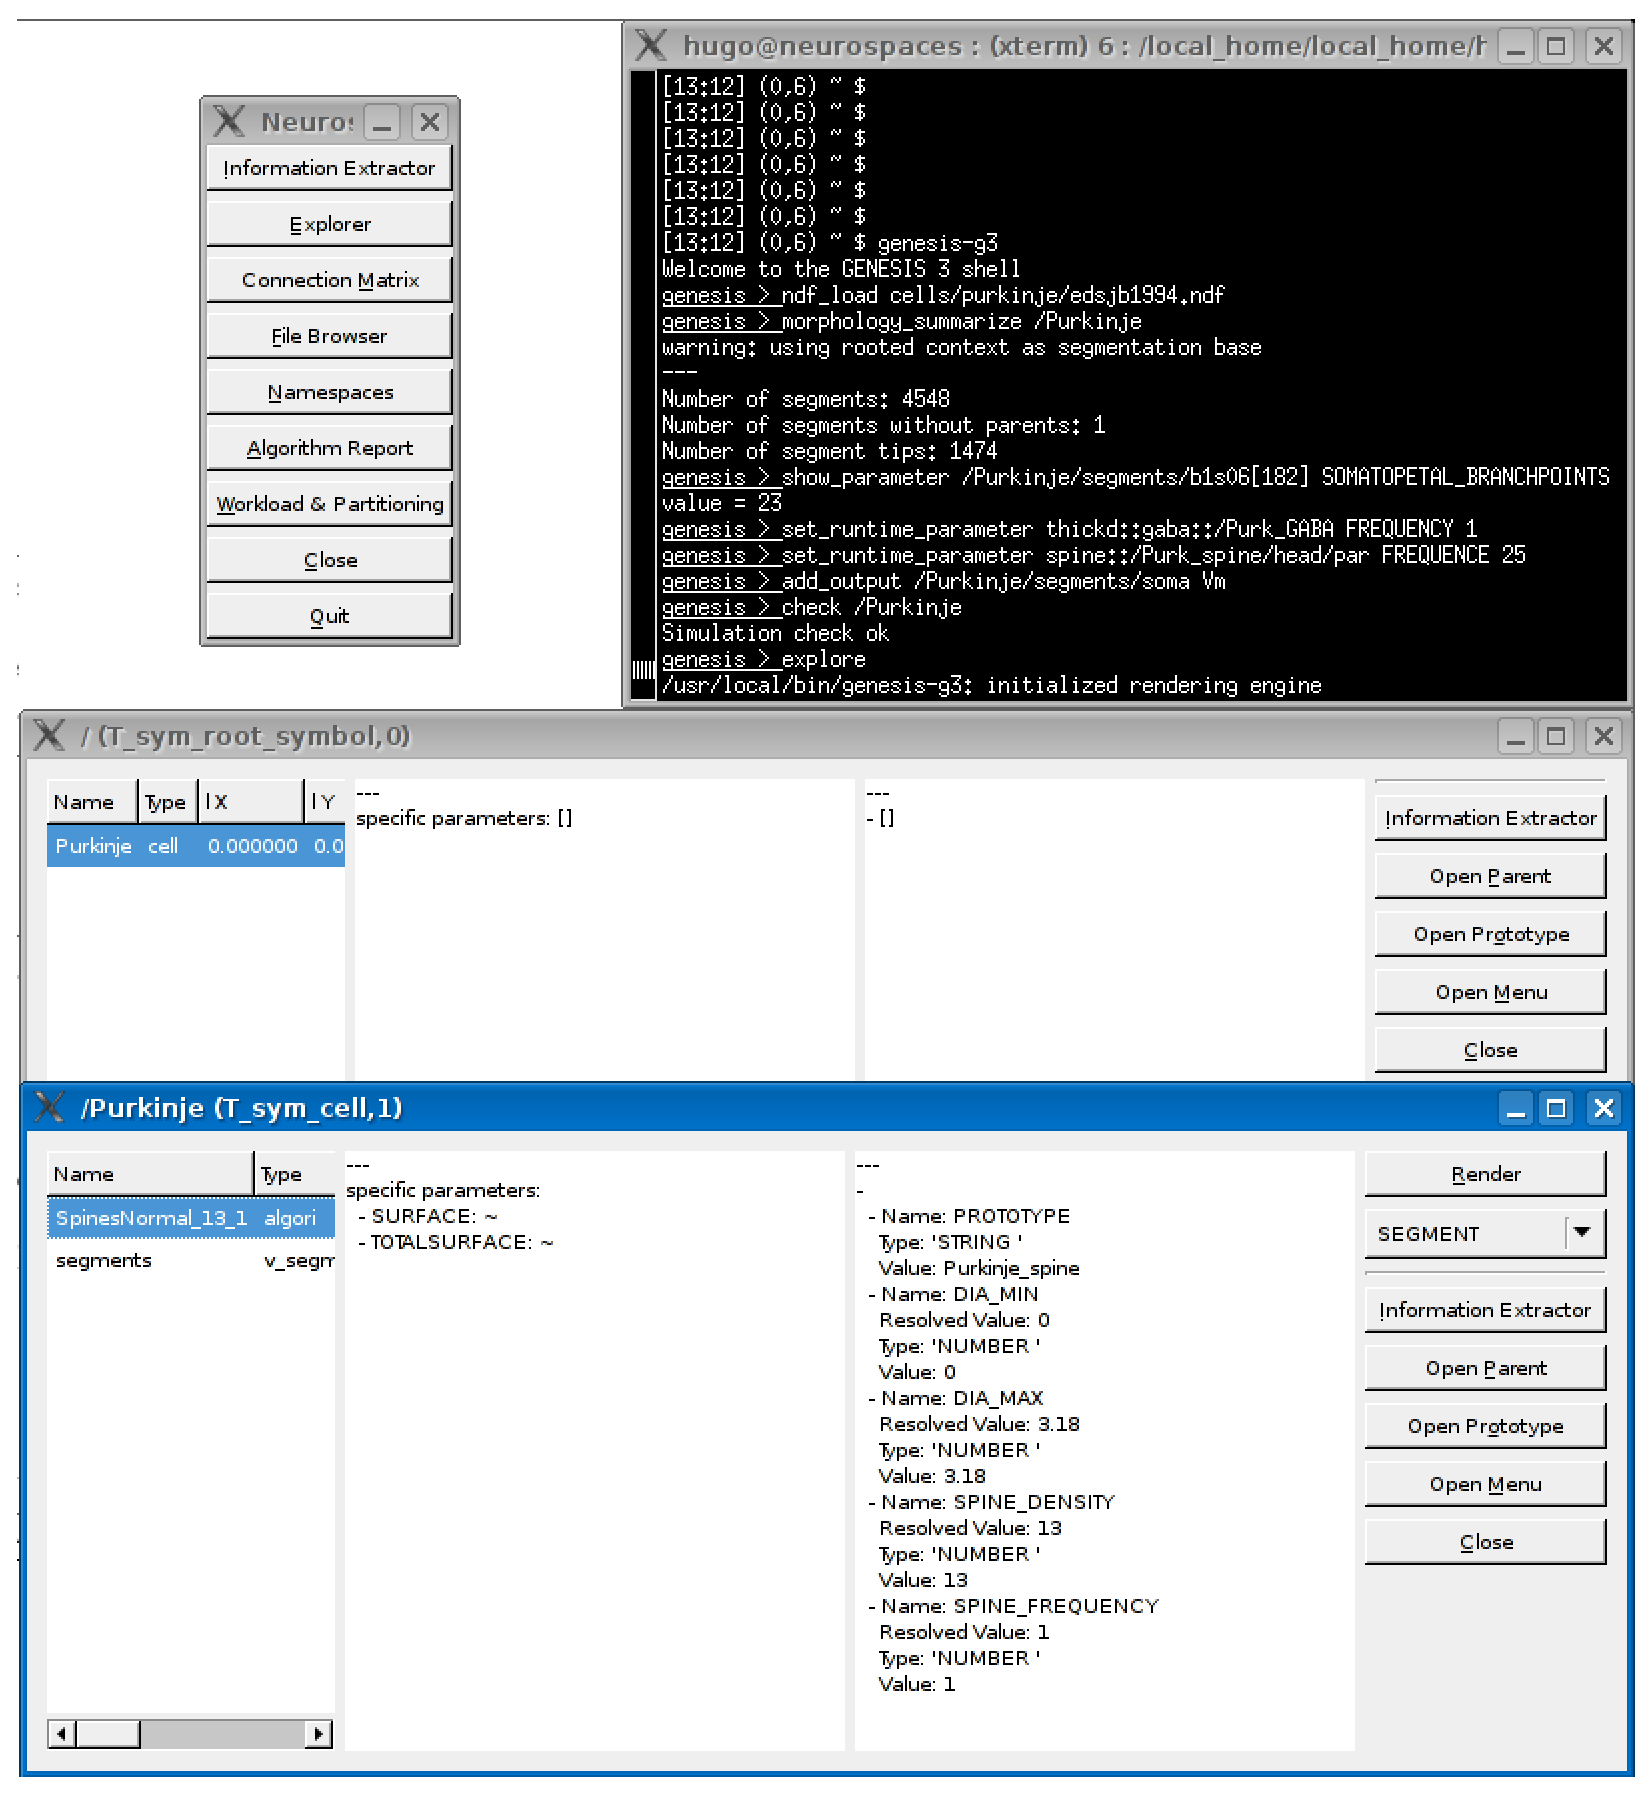
\includegraphics[scale=0.3]{figures/studio-screenshot.eps}
  \caption{Using the Neurospaces Studio to Query a Model and its
    Parameters}
  \label{fig:cbi-studio}
\end{figure}


Given the name of one of its dendritic segments, the number of branch
points between that segment and the soma can be determined. After
indicating which paths of the dendritic tree must be examined, the
parameter {\tt SOMATOPETAL\_BRANCHPOINTS} contains the result, which
can be obtained with:

{\footnotesize
\begin{verbatim}
morphology_summarize /Purkinje
show_parameter /Purkinje/segments/b1s06[182] SOMATOPETAL_BRANCHPOINTS
\end{verbatim}
}

After finding a suitable dendritic segment, its synaptic channel can
be stimulated with a precomputed spike train using:

{\footnotesize
\begin{verbatim}
set_runtime_parameter /Purkinje/segments/b1s06[182]/Purkinje_spine_0/head/par/synapse EVENT_FILENAME ``event_data/events.yml''
\end{verbatim}

Finally, a simulation can be conveniently started using:

{\footnotesize
\begin{verbatim}
add_output /Purkinje/segments/soma Vm
run /Purkinje 0.1
\end{verbatim}
}

This outputs the soma membrane potential to a file with a default
filename of {\tt /tmp/output}.


\subsection{Gluing Pre-existing Applications \& Libraries}

As mentioned above, one advantage of the CBI federated software
architecture is that it defines how to interface simulator components
with external applications.  An obvious example is the use of existing
3D graphics software to examine and edit the spatial properties of a
model neuron morphology.  Others include, integration with external
graphing and windowing software for plotting the values of solved
variables against simulation time, or to allow the construction of
button rich tutorial applications.

We are currently working on integration of the G3 platform and the WX
library to build cross platform GUIs using the Python module {\it
  wxPython}.  {\it matplotlib} is a Python interface to a 2D plotting
library producing publication quality figures in a variety of hardcopy
formats.

All these libraries exist and are publicly available for download,
however, they must be provided with data bindings such that, for
example, the data produced by a mathematical solver flows to a widget
that plots the value of a variable against time.  The events that are
generated inside such a GUI application fall into one of two
categories.  The first, considers events generated to open a menu or
dialog interface.  The second, considers events that interact with the
simulation.  Since a lot of documentation for the former is available
on the internet, we only deal here with the latter, and focus on
events such as starting and stopping a simulation.

Most contemporary GUI applications are conveniently constructed using
one of the available user interface builders.  wxFormBuilder
(http://wxformbuilder.org/; a user interface designer for the wxPython
toolkit and the Linux desktop environment GNOME) is one such builder.
It allows the user to construct a GUI with visual elements such as
menus and buttons, and write a description of the elements to an XML
file that is readable via Python bindings.

%What remains to be done is the binding of button events to specific
%actions for the simulator.

%Because the focus of Glade is simple GUI applications, it does not
%directly support plotting functions.  In our example we choose to
%imported these from the {\it matplotlib} library.

In the examples below, we show Python scripting to connect the
software components required to build a small GUI for the G3
simulator.  For this, we assume that a wxFormBuilder file with name
{\tt G3.wx} can be found that describes a GUI with one window (name:
window1), allows the simulation duration to be set, and contains a
button to start the simulation.

The first lines of code in the script load the necessary Python
modules which in turn load libraries coded in a low-level system
programming language.

{\footnotesize
  \resetlinenumber
  \linenumbers
\begin{verbatim}
import wx
\end{verbatim}
}

The following Python code reads the Glade XML file and connects a
button with a function to run the simulation:

{\footnotesize
  \resetlinenumber[5]
  \linenumbers
\begin{verbatim}
wTree = gtk.glade.XML("G3.glade", "window1")
wTree.signal_autoconnect( { "on_button1_clicked": run_simulation } )
\end{verbatim}
}

The function {\it run\_simulation} is a Python function with a
function body that contains a complete listing of the first Python
example (above). The {\it edit} field with the simulation time
requires the use of a global variable that follows the value in that
field:

{\footnotesize
  \resetlinenumber[8]
  \linenumbers
\begin{verbatim}
def set_simulation_time(self):
    global simulation_time
    simulation_time = self.get_text()
    
wTree.signal_autoconnect
      ( { "on_simulation_time_changed": set_simulation_time } )
\end{verbatim}
}

The code of a GUI application is always terminated by a call to the
main event loop of the GUI library.

{\footnotesize
  \resetlinenumber[14]
  \linenumbers
\begin{verbatim}
gtk.main()
\end{verbatim}
}

This script runs a small model and can be combined with other Python
code given here to increase the complexity of a model, add various
stimulus conditions, and extract the output of interest.  The script
saves the membrane potential of the soma to the file {\tt
  /tmp/output}.  To plot this membrane potential in the application
window, the {\it matplotlib} library is used:

{\footnotesize
  \resetlinenumber[5]
%  \linenumbers
\begin{verbatim}
import matplotlib
import pylab
\end{verbatim}
}

The following code reads the output file into two arrays, {\tt t} and
{\tt v}:

{\footnotesize
  \resetlinenumber[5]
%  \linenumbers
\begin{verbatim}
    t = []; v = [] ;
    file = open("/tmp/output")
    for line in file:
        values = re.split(" ", line)
        t.append(float(values[0]))
        v.append(float(values[1]))
\end{verbatim}
}

The plot widget is not directly supported by Glade and must be created
with custom Python code.  A plot can then be generated using:

{\footnotesize
  \resetlinenumber[5]
%  \linenumbers
\begin{verbatim}
    # generate the plot
    figure = matplotlib.figure.Figure(figsize=(6,4), dpi=60)
    axis = figure.add_subplot(111)
    axis.plot(t,v)

    # display the plot
    canvas = matplotlib.backends.backend_gtk.FigureCanvasGTK(figure)
    canvas.show()
    grahview = wTree.get_widget("vbox1")
    grahview.pack_start(canvas, True, True)
\end{verbatim}
}

A more complex example illustrates the integration of G3 with Blender
(http://www.blender.org/, a free open source 3D content creation suite
with an active developer community and available for all major
operating systems that have Python enabled bindings\,\footnote{Blender
  has the restriction that the Python code must be run from the
  Blender Python interpreter.}) to validate and analyze models of the
morphology of small dendritic segments obtained from electron
microscopy data. Past research on cerebellar Purkinje cells has shown
that the balance between excitation and inhibition plays an important
role in dendritic processing\,\cite{santamaria02:_modul_purkin,
  mittmann07:_linkin_purkin}.  However, the spatial resolution of the
models employed in such studies was limited by the reconstruction
techniques then available.  Consequently, over the last several years
we have used electron microscopy in conjunction with
Reconstruct\,\cite{jc05:_recon}
% (Fiala, 2005;
%http://www.bu.edu/neural/Reconstruct.html, a Windows based application
%for montaging, aligning, tracing, measuring, and reconstructing
%objects from serial section images)
% \marginpar{cite howard}
to obtain more precise morphologies of small segments of Purkinje cell
dendrite\,\cite{lu09:_d_purkin, cornelis08:_model_neuros_genes}).
%Fiala JC (2005) Reconstruct: a free editor for serial section microscopy. J Microscopy 218:52-61.

\begin{figure}[ht]
  \centering
    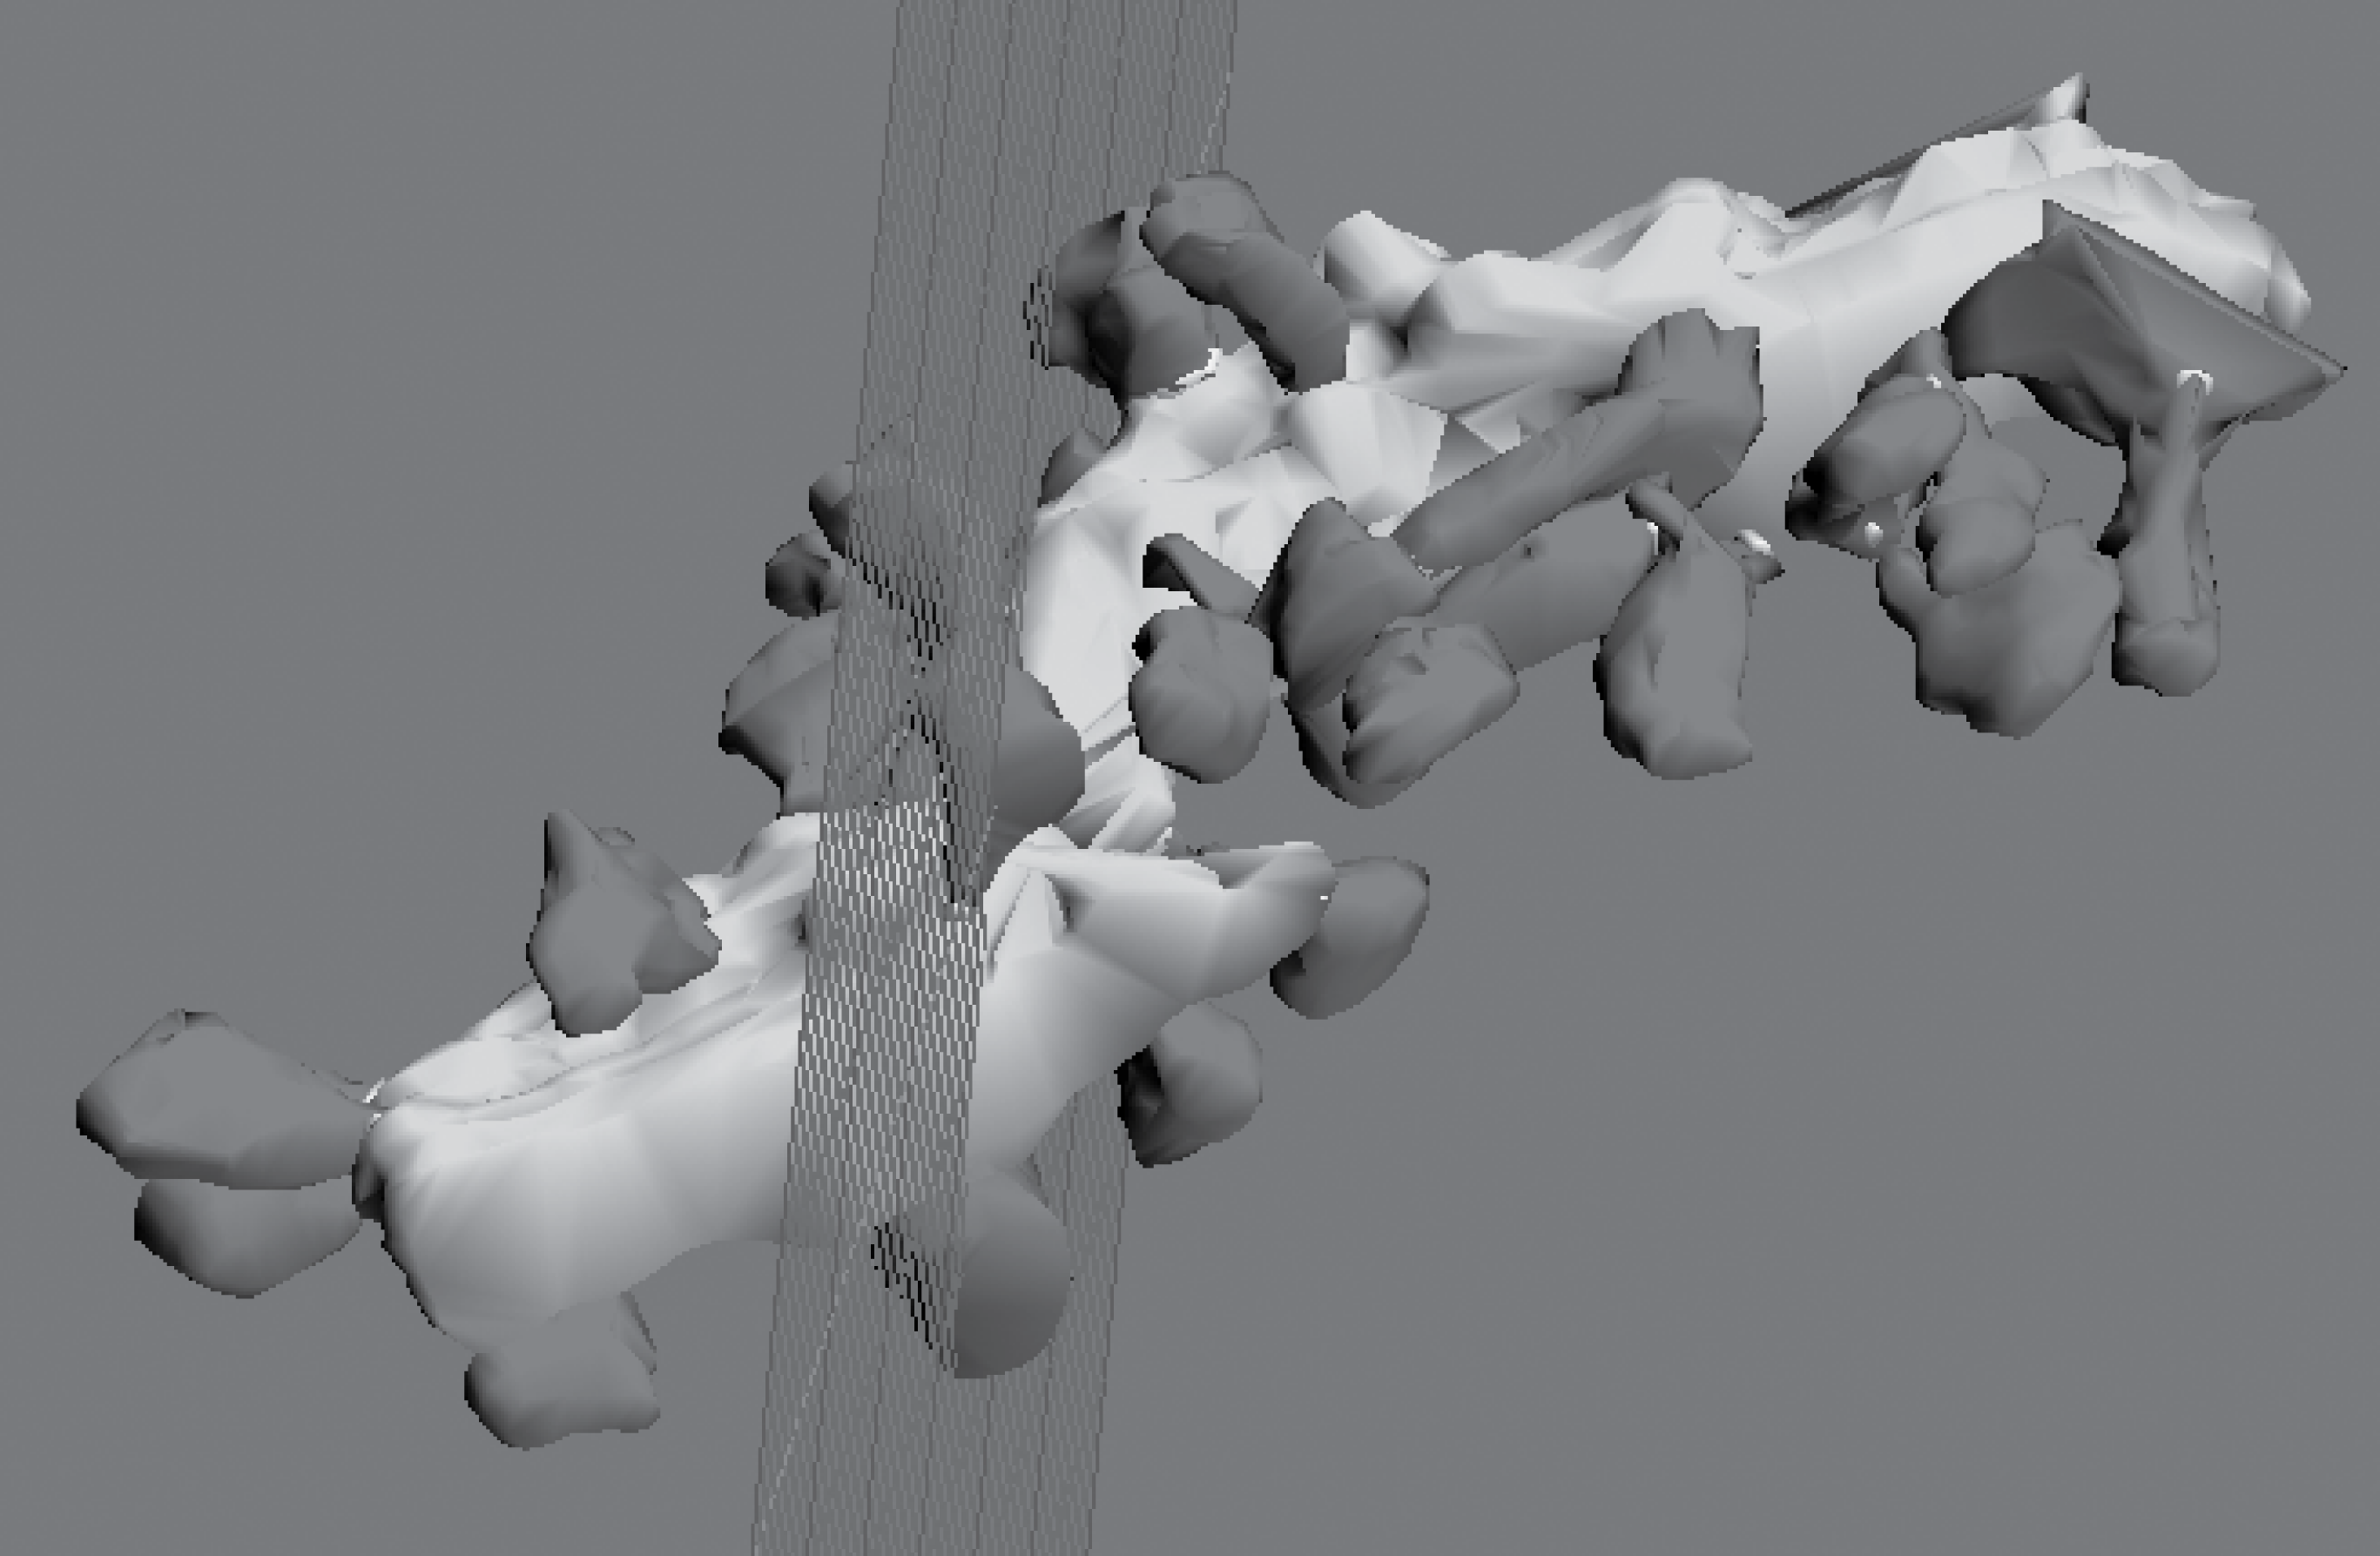
\includegraphics[scale=0.5]{figures/blender-python-bw.eps}
  \caption{Blender image of Purkinje neuron dendritic segment}
  \label{fig:cbi-blender}
\end{figure}

%Show Python interface snippet.

Special purpose software has been written to convert Reconstruct data
for importation into the G3 model container.  The core of these
algorithms implements geometrical transformations such that EM
contours are extracted to provide equivalent cylinders suitable for
cable modeling.  The geometrical properties of the cylinders are
stored as NDF files (the file format used by G3), and algorithms
provided by the model container link them with the cable parameters
required by the mathematical solvers.  A simulation can then be run
with the {\it read} and {\it run} methods mentioned above.

The necessary conversion algorithms are accessible from Python via the
model container.  The Python interface of Blender links it to the G3
simulator, such that Blender becomes the first 3D model inspection
tool for EM data.  As an example, the Python script developed above
can be run from within the Blender environment.  Also, via the same
Python interface simulations can be started based on the 3D image
data.

Interactive visualization of reconstructed dendritic segments is a
valuable method of model validation and is available with the
interface of G3 and Blender (see Figure~\ref{fig:cbi-blender}).
However, the development of small focused plugins allows for more than
just these functions. For example, 3D measurement and manipulation of
neuron morphology, computation of surface areas and volumes, and the
generation of 3D crossections and 2D cuts.

\subsection{Future Directions}
Complementary functionality to that provided by interfacing G3 with
Blender would be available after interfacing G3 with {\it
  neuro}Construct, a software package designed to simplify development
of complex networks of biologically realistic
neurons\,\cite{gleeson05:_build_networ_model}.  Implemented in Java,
it can be connected to Python applications (e.g. see
http://www.jython.org/).  {\it neuro}Construct uses the latest NeuroML
specifications (see http://www.neuroml.org), including MorphML
(http://www.morphml.org/), ChannelML (part of Level 2 of the NeuroML
set of standards) and NetworkML (the core of NeuroML Level 3) and can
be used to visually validate network layout and
design\,\cite{crook07:_morph}.
% [135]  P. Gleeson, V. Steuber and R. A. Silver (2007) neuroConstruct: A Tool for Modeling Networks of Neurons in 3D Space, Neuron, 54: 219-235.

Finally, we note that we have developed a serial communication
framework for event delivery of action potentials to postsynaptic
targets (DES: Discrete Event System).  This software component is
integrated with the mathematical solvers of G3 using either Python or
Perl.  Because it is optimized for communication over serial hardware,
we plan to extend it with communication frameworks for parallel
hardware such as that provided by the MOOSE simulator (see Ray and
Bhalla, this issue) and the MUSIC
framework\,\cite{ekeberg08:_music_multis_coord}.


\vspace*{-4mm}
\section{Conclusion}

Software libraries can be divided into application specific and
application neutral categories.  The Neurospaces project provides a
series of software components specific to neuroscience applications.
The advantage is that a scripting language such as Python becomes a
powerful integration tool to connect these components to general
purpose libraries for visualization, rendering, and GUIs.  A key
enabling property of G3 is that it stores model parameters separately
from stimulation protocols and the way simulations are run.  By
defining clear functional boundaries of the core software components
such as the model container and the mathematical solvers, we also
provide clear interfaces for integration.

Although the Python bindings of the G3 simulator embed the same
powerful concepts as the GENESIS SLI, their purpose is different.
While the SLI had as major goals the integration of model components,
output collection, and running simulations, the primary goal of
scripting languages such as Python has become application integration.

Here, we have illustrated the relationship between Python and the G3
simulator.  We have focused on a simple but comprehensive example, the
running of a single compartment neuron and the plotting of its
membrane potential. The purpose is to demonstrate the advantages of
using high-level scripting languages such as Python for binding the
independent stand-alone components of G3.

%It is an approach that
%simplifies the extension, modification, and customization of the
%GENESIS platform, not only for developers but also most importantly
%for users.

We are currently using Blender for visual inspection and validation of
reconstructed dendrites by connecting the model to the geometrical and
analytical tools provided by the Blender plugin library.  However it
is also possible to use Blender to instantiate neural simulations,
and, as an example, to collect the output data for movie generation.
%, and the
%simulation to movie generation and other relevant functions provided
%by the Blender plugin library.
Employed in this way, the modularized design of the G3 simulator
provides for progressive federated software development.

%The G3 platform uses scripting to connect neuroscience specific
%software to general purpose software and integrate it into a next
%generation simulator.  The advantage is that third party software
%libraries and applications become available for users, for example,
%Blender, {\it matplotlib}, and Glade, among many others. This has
%become possible due to the rearchitectured GENESIS software design
%where G3 now stores model parameters separately from stimulation
%protocols and the way simulations are run. It is the stand-alone
%nature of the individual software components and the fact that they
%can now easily be interfaced that serves the purpose of continued
%development and user-friendliness.
%Using Python for integration makes
%the application much more accessible to users.


% ********************** Back matter ********************************
% Bibliography
\cleardoublepage
\pagenumbering{roman}
\bibliographystyle{abbrv}
%\bibliography{DDDAS_bib_library}
%\bibliography{crest2008,Qian,DDDAS_bib_library}
\bibliography{all}

% ********************** End of the Document ************************
\end{document}


%%% Local Variables: 
%%% mode: latex
%%% TeX-master: t
%%% End: 
